\section*{Expulsion: Propagation of Deletions and Selective Sync}
\label{sec:expulsion}

The system propagates file and folder deletion updates among devices as one type
of object update. Users are additionally permitted to specify those files and
folders which they would not like to sync to a particular device (but which
remain synchronized among all other devices). Common to both features is the
method of labeling a file or folder as {\em expelled}. Among other data stored
in the logical representation of the file system (e.g. name, object id), the
system stores a boolean expelled flag for each object.

\subsection*{Expulsion: Selective Sync}
Initially all new objects are flagged as false ({\em admitted}). To unsync a
file at the local device, the expelled flag is set to true, and the file is
consequently deleted from the physical file system, without incrementing
versions in the consistency algorithm (i.e. do not create an update about this
deletion). To unsync a directory, it is flagged as expelled, along with all
descendent files and directories in the logical file system. The aforementioned
physical files/directories are deleted. If the parent directory of an object is
expelled, then that child object must necessarily be expelled as well. No
versions are incremented in the consistency algorithm when a folder and its
children are expelled; this is a local operation, not to be shared with other
devices.

%TODO is this sufficient for a patent? I've effectively described the ``basic
%idea," and some invariants. Those are more like tools for a proof, not an
%algorithm or method.
%TODO is a figure needed to explain the expelled bit? and selective sync?

\subsection*{Deletion propagation via a logical trash folder}

\begin{figure}[t]
\centering
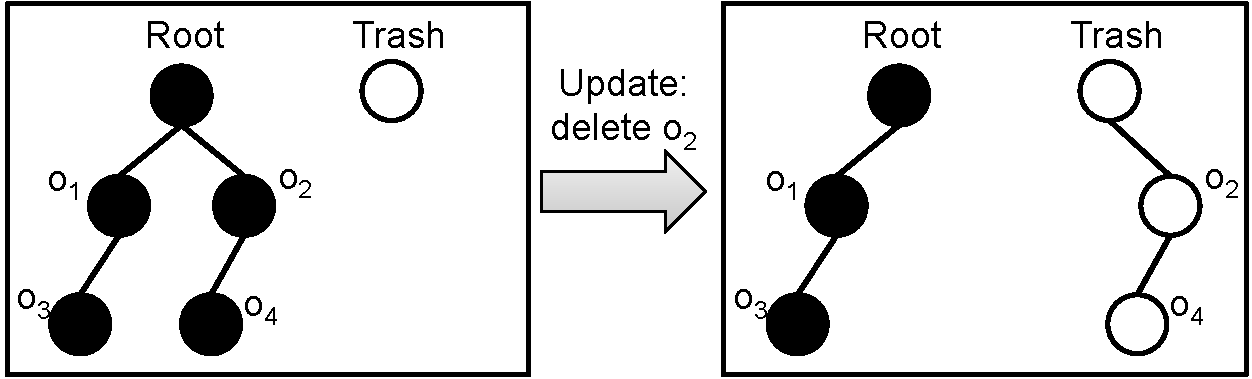
\includegraphics[width=\textwidth]{figs/trash.pdf}
\caption{Updating the logical file system on deletion by moving to the Trash
Folder}
\label{fig:trashfolder}
\end{figure}

Unlike selective sync, where an object is physically deleted on only one device,
but synced among all others, the system additionally supports the propagation of
deletions. This feature relies on a special directory that is expelled in
every store, known as the {trash folder}, shown in
Figure~\ref{fig:trashfolder}. Pictured in the left box of the figure is a tree
representation of the logical directory tree. Tree nodes are logical objects
representing directories or files; nodes with children are necessarily
directories on the physical file system. For example, the node labeled ``Root"
is the root directory of the store, with two children directories $o_1$
and $o_2$, which have one child object each, $o_3$ and $o_4$, respectively.
Empty (or white) nodes represent expelled objects, and full nodes are not
expelled. The trash folder is always marked expelled, thus it appears only in
the logical file tree, not on the physical file system. In every store,
on every device, the trash folder has the same object id.

To propagate a deletion update for an object, the object is moved to the trash
folder. This is demonstrated in Figure~\ref{fig:trashfolder}. In the initial
state (on the left) directory $o_2$ was under the root directory. The system
is notified that, locally, $o_2$ has been deleted. Thus $o_2$ is logically moved
under the trash folder. Because children of an expelled folder are also
expelled, $o_2$ and its children are expelled. As with all object moves, the
logical movement of $o_2$ to the trash folder warrants a version increment for
$o_2$ in the consistency algorithm. Via the Collector algorithm, remote devices
will collect the update that $o_2$ has been moved under the trash folder. Thus
they will set the expelled flag on $o_2$ after moving it under the trash folder,
and delete it from the physical file system. Hence, object deletions are
propagated by logically moving objects under the known, expelled trash folder.

%TODO explain that local versions of content for files are moved to kml? That
%would require explaining meta and content components.
% - the components are explained in the base patent
%
%TODO explain that metadata is kept in O table, but content attributes are
%deleted?
